\chapter{Estimation of Active Sources}
In this chapter the issue of unknown $k$ is considered. The aim is to investigate the possibility of identifying an estimation of a non-active source signal from $\hat{\textbf{X}}_{Main}$ when the true $k$ is not provided to the algorithm. Instead of providing the true $k$ one let $k=N$ as such one ask the algorithm for $N$ non-zero source signals, but there only $k<N$ non-zero source signal within the synthetic data set. 

Figure \ref{fig:ktest1} visualise the estimate $\hat{\textbf{X}}_{Main}$ from a stochastic data set $\textbf{Y}$ specified by $M=N=8$, $k=4$ and $L=1000$. 
As seen i section \ref{sec:testMsbl_stoch} the case of $M=N$ should be solved almost exact by the M-SBL algorithm with true $\textbf{A}$ given. From the figure it is seen that the estimates of the zero rows have amplitudes close to zero, which distinguishes them from the remaining exact estimates. Due to the estimates of the zero row being this close to zero they do not affect the MSE which is close to zero, thus do not indicate flaws within the estimate. 
Furthermore it seen that the estimates of the zero rows form a scaled copy of one of the exact estimates. These observation indicates that it is possible to distinguish the estimates of non-zero rows.     

\begin{figure}[H]
    \centering
	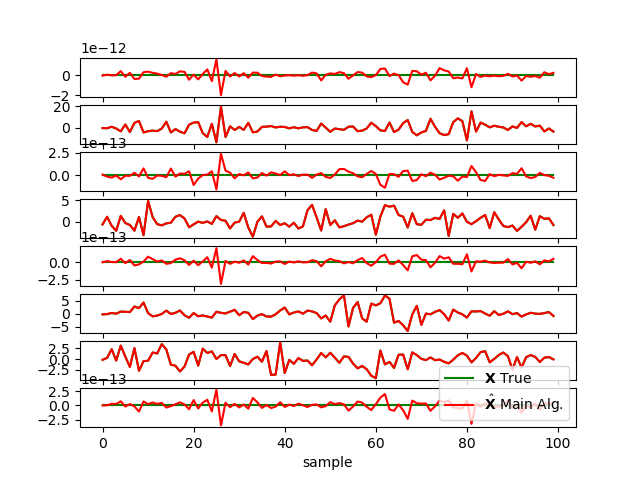
\includegraphics[scale=0.5]{figures/ch_estimate/k_test1.png}
	\caption{MSE is 1.196e-29}
	\label{fig:ktest1}
\end{figure}

Consider now the case where desired case where $M<N$. 
As a reference figure \ref{fig:ktest2} visualise the estimate $\hat{\textbf{X}}_{Main}$ from a stochastic data set $\textbf{Y}$ specified by $M=6$,$N=8$,$k=8$ and $L=1000$.  
Now the true $k$ is reduced, and the estimate is computed again.
Figure \ref{fig:ktest3} visualise the estimate $\hat{\textbf{X}}_{Main}$ from a stochastic data set $\textbf{Y}$ specified by $M=6$,$N=8$,$k=4$ and $L=1000$.
From figure \ref{fig:ktest3} it is now seen that the estimates of the zero rows is not as close to zero as in figure \ref{fig:ktest1}. Thus this can not be used as the indicator. However, the estimates of the zero rows still appears as a scaled copy of an estimate of a non-zero row. One attempt to locate the zero rows is to compare each row of $\hat{\textbf{X}}_{Main}$ to ever other row by the MSE, in order to check if it appears more than one time
Two rows are considered replicas if the mutual MSE is below a tolerance equal to 1. This operation is performed on the estimate plotted in figure \ref{fig:ktest3} gives the result displayed in table \ref{tab:replica1}

\begin{table}[h]
\begin{tabular}{|l|l|l|l|l|l|l|l|l|}
\hline
row index   & 1 & 2 & 3 & 4 & 5 & 6 & 7 & 8 \\ \hline
\# replicas & 4 & 4 & 1 & 4 & 1 & 1 & 1 & 4 \\ \hline
\end{tabular}
\caption{•}
\label{tab:replica1}
\end{table}

\begin{figure}[H]
    \begin{minipage}[t]{.45\textwidth}
		\centering
		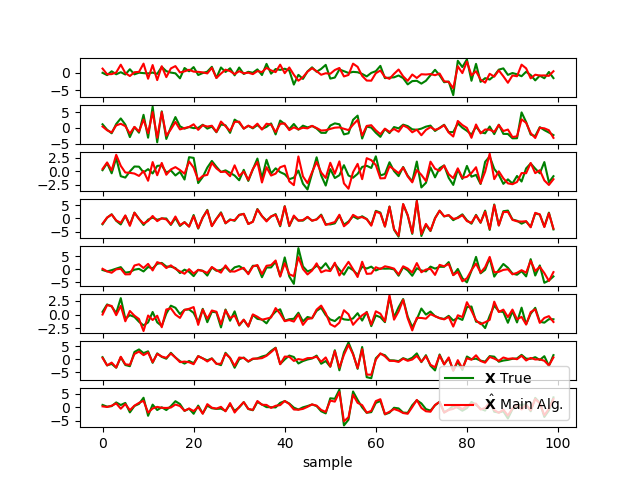
\includegraphics[scale=0.5]{figures/ch_estimate/k_test2.png}
	\caption{M=6, N=k=8, L=1000, MSE is 1.189}
	\label{fig:ktest2}
    \end{minipage} 
    \hfill
    \begin{minipage}[t]{.45\textwidth}
		\centering
		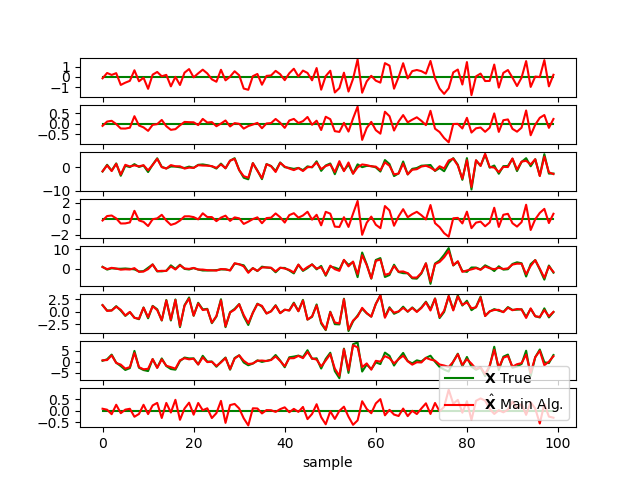
\includegraphics[scale=0.5]{figures/ch_estimate/k_test3.png}
	\caption{M=6, N=8, k=4, L=1000, MSE is 0.344}
	\label{fig:ktest3}
    \end{minipage}
\end{figure}

now let $\textbf{A} = \textbf{A}_{fix}$ 


\begin{figure}[H]
    \begin{minipage}[t]{.45\textwidth}
		\centering
		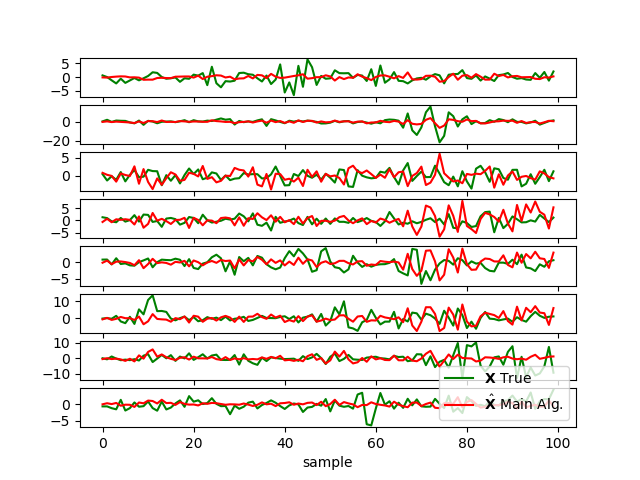
\includegraphics[scale=0.5]{figures/ch_estimate/k_test4.png}
	\caption{}
	\label{fig:ktest4}
    \end{minipage} 
    \hfill
    \begin{minipage}[t]{.45\textwidth}
		\centering
		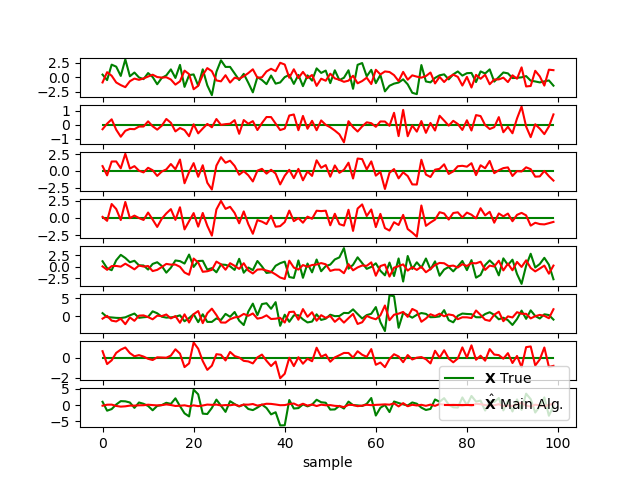
\includegraphics[scale=0.5]{figures/ch_estimate/k_test5.png}
	\caption{}
	\label{fig:ktest5}
    \end{minipage}
\end{figure}
